\documentclass{article}

% pacchetti
\usepackage[utf8]{inputenc} 
\usepackage[italian]{babel}
\usepackage{url}
\usepackage{hyperref}
\usepackage{xcolor}
\usepackage{graphicx} % per le immagini
\usepackage{amsthm}
\usepackage{amsmath}
\usepackage{amssymb}
\usepackage{wrapfig} % per le immagini incorniciate con il testo
\usepackage{fancyhdr} % per i headings e footers
\usepackage{eurosym} % per il simbolo dell'euro "€" più carino
\usepackage{appendix}
\usepackage{geometry}
\usepackage{extpfeil}
\usepackage{tikz}
%\usetikzlibrary{patterns,plotmarks} %per usare root con tikz
\usepackage{multirow}
\usepackage{multicol} % per avere elenchi a più colonne
\usepackage{enumitem}
\usepackage{soul} % per highlight migliore

\usepackage{minted}
\definecolor{bg}{rgb}{0.95,0.95,0.95}
\definecolor{green}{rgb}{0,.66,0}
\definecolor{white}{rgb}{1, 1, 1}


% impostazioni del pacchetto fancyhdr
\pagestyle{fancy}
\fancyhf{}
\rhead{\sc ye leandro}
\lhead{Relazione \texttt{ROOT\textunderscore project}}
\fancyfoot[c]{\thepage}

\begin{document}


%\thispagestyle{plain} % per ignorare per questa pagina le impostazioni fancy
\thispagestyle{empty} % per disattivare per questa pagina le impostazioni fancy e anche il numero della pagina

\begin{figure}[h]
    \centering
    \includegraphics[width=0.5\textwidth]{image/logo.png}
    \label{Logo}
\end{figure}

\vspace{2cm}

\section*{\centering \Huge \bf Relazione \texttt{ROOT\textunderscore project}}

\vspace{3cm}

\begin{center}
{\large Realizzato da} \\
\vspace{2cm}
{\Large \textsc{Leandro Ye}}    
\end{center}

\vspace{3cm}

\begin{center}
    {\large 8 aprile 2023}
\end{center}

\newpage

\section{Introduzione}

Nella seguente relazione si intende simulare eventi di collisioni tra vari tipi di particelle e fare analisi di dati a riguardo. Per la realizzazione del programma si è utilizzato il linguaggio C++ con la libreria ROOT, con particolare enfasi sulla programmazione ad oggetti, sulla simulazione di eventi fisici tramite generazione Monte Carlo e infine sull'analisi con ROOT.\\

I tipi di particelle coinvolte posso essere raggruppati in due categorie: quelli stabili e quelli molto instabili, ossia risonanze. Per lo scopo di questo progetto, di queste particelle andiamo a considerare solo queste caratteristiche: massa, carica, quantità di moto. Solo alle risonanze però si associa un'altra caratteristica, la larghezza di risonanza. Inoltre le particelle considerate sono: pioni ($\pi^\pm$), kaoni (K$^\pm$), protoni (p$^\pm$) e infine K$^*$, con K$^*$ la particella di risonanza. \\

Nel corso delle interazioni tra queste particelle, emergeranno i parametri di K$^*$, e lo scopo di questo progetto è riuscire a determinare questi parametri.\\

\section{Struttura del codice} 

In questo progetto si è andati ad utilizzare la programmazione ad oggetti, e più in particolare l'\textbf{ereditarietà virtuale} e l'\textbf{aggregazione}.

\subsection*{Le classi \texttt{ParticleType} e \texttt{ResonanceType}}
Nella simulazione si hanno due categorie di particelle: quelli ordinari e le risonanze. Avendo queste ultime una caratteristica aggiuntiva rispetto a quelle ordinarie (cioè la larghezza di risonanza), allora si è pensato di creare una classe \verb|ParticleType| associato ai tipi particelle ordinarie e da questa si è andati a ereditare la classe \verb|ResonanceType|, associata alla tipologia di risonanza. \verb|ParticleType| possiede \textbf{tre attributi privati}:
\begin{itemize}
    \item \verb|std::string fName|: indica il \textbf{nome} del tipo di particella;
    \item \verb|double fMass|: indica il valore di \textbf{massa} (in GeV/c$^2$);
    \item \verb|int fCharge|: indica il valore di \textbf{carica} ($\pm$\textit{e}).
\end{itemize}
\verb|ResonanceType| include anche l'attributo privato \verb|double fWidth| che indica la \textbf{larghezza}.\\
Per ognuno di questi parametri c'è un metodo che ritorna il valore se richiesto (\verb|GetName()|, \verb|GetMass()|, \verb|GetCharge()|, \verb|GetWidth()|).

\subsection*{La classe \texttt{Particle}}

Alla generazione di una particella dobbiamo specificare le sue caratteristiche di base e le proprietà cinematiche (quantità di moto e direzione). Per far ciò si potrebbero attribuire le singole caratteristiche associato al tipo di particella, ma ciò è dispendioso per la memoria ed è meglio attribuire semplicemente il tipo di particella.\\

Utilizzando l'aggregazione del codice si è creato una classe \verb|Particle| che descrive queste caratteristiche, contenendo in privato:
\begin{itemize}
    \item \verb|static std::vector<ParticleType> fParticleType|: una \textbf{lista} (contenitore) di tutti i tipi di particelle creati;
    \item \verb|int fIndex|: un \textbf{numero} che identifica la tipologia di particella in base alla sua posizione in \verb|fParticleType|;
    \item \verb|Vector3d fImpulse|: un \textbf{vettore 3-dim} che racchiude i tre componenti dell'impulso.
\end{itemize}
Inoltre in questa classe troviamo diversi metodi, sia privati che pubblici:
\begin{itemize}
    \item metodi che ritornano i parametri singoli della particella corrente (indice del tipo di particella, vettore dell'impulso, massa, carica);
    \item metodi che impostano i parametri alla particella corrente (tipo di particella, impulso);
    \item \verb|int FindParticle(...)|: ritorna l'indice del tipo della particella in base al nome dato in input;
    \item \verb|void AddParticleType(...)|: aggiunge un tipo di particella in \verb|fParticleType|;
    \item \verb|double GetEnergy()|: ritorna il valore dell'energia della particella corrente, secondo l'equazione
    
    $$ E = \sqrt{m^2 + |\Vec{p}|^2} $$
    
    con $E$ l'energia, $m$ la massa, $|\Vec{p}|$ il modulo dell'impulso;
    \item \verb|double InvMass(...)|: ritorna il valore della massa invariante tra quella corrente e un'altra particella, secondo
    
    $$ M_{inv} = \sqrt{(E_1 + E_2)^2 - (\vec{p_1} + \vec{p_2})^2} $$
    
    con $M_{inv}$ la massa invariante, $E_i$ e $\Vec{p_i}$ rispettivamente l'energia e vettore dell'impulso della particella $i$;
    \item \verb|double Decay2Body(...)|: simula il decadimento della particella corrente in altre due; 
\end{itemize}

Un altro punto fondamentale di questo progetto è la \textbf{modularità} del codice: per ogni classe sono stati definiti un file di intestazione e uno d'implementazione (quindi 6 file complessivamente), che, una volta compilati, sono stati resi come librerie dinamiche per un maggior efficacia nel fase del linking.\\

\subsection*{Il file \texttt{main.cpp}}

Le librerie create sono stati utilizzati nel file \verb|main.cpp|, in cui si esegue la parte di simulazione del programma.\\
Ciò consiste in simulazione di eventi di collisione in cui vengono generati un numero fisso di particelle (\verb|Particle|) per evento. Per ogni generazione di  particella le vengono attribuite casualmente un impulso con direzione e verso (\verb|fImpulse|), le viene assegnato la tipologia di particella (\verb|fIndex|) secondo una distribuzione definita dall'utente e infine, se viene generato una risonanza, questa viene fatto decadere in altre due.\\
Durante le generazioni in un evento vengono raccolti dati in istogrammi che poi andranno ad essere analizzati successivamente. I dati che vengono raccolti di una particella generata sono il tipo di particella, la distribuzione degli angoli dell'impulso (azimutale e polare), il modulo dell'impulso totale e trasversa e l'energia. Alla fine di un evento vengono valutati anche le masse invarianti tra le particelle, in particolare quelle derivanti tra tutte le particelle, tra tutte le particelle di segno concorde e di segno opposto, tra particelle K e $\pi$ di segno concorde  e di segno opposto e infine tra particelle entrambi generate da uno stesso decadimento di un K$^*$. 
Alla fine dell'esecuzione del programma vengono mostrati e salvati i dati della simulazione effettuata.\\

\subsection*{Il file \texttt{analytics.cpp}}
Infine, una volta salvati i dati della simulazione, questi vengono analizzati e fittati.
In particolare vengono analizzati e valutati il numero di particelle generati per tipo, i parametri della particella (angoli e modulo dell'impulso) e le masse invarianti. Da queste analisi si cerca di rilevare il segnale di K$^*$ che verrà generato con frequenza molto minore rispetto ad altre particelle.\\

\section{Generazione}

Nel programma vengono generati 10 000 eventi, in ognuno dei quali vengono generati 100 particelle.\\
Le particelle in totale sono 7, con i tipi, le caratteristiche e la distribuzione delle particelle generate raccolte nella tabella \ref{tab:particles}.

\begin{table}[htp]
    \centering
    \begin{tabular}{||c|c|c|c|c||}
        \hline \hline
        \multicolumn{5}{||c||}{\textsc{tipo, caratteristiche e distribuzione delle particelle}} \\
        \hline \hline
        tipo & presenza & massa [GeV/c$^2$] & carica [$e$] & larghezza [GeV/c$^2$]\\
        \hline
        $\pi^\pm$ & 40\% & 0.13957 & $\pm1$ & $-$\\
        K$^\pm$ & 5\% & 0.49367 & $\pm1$ & $-$\\
        p$^\pm$ & 4.5\% & 0.93827 & $\pm1$ & $-$\\
        K$^*$ & 1\% & 0.89166 & 0 & 0.050\\
        \hline \hline 
    \end{tabular}
    \caption[\small Tipo, caratteristiche e distribuzione delle particelle]{\small Il tipo, le caratteristiche e la loro distribuzione nelle simulazioni, con $\pi^\pm$ pioni, K$^\pm$ kaoni, p$^\pm$ protoni e  K$^*$ la particella di risonanza. La sezione "presenza" indica la distribuzione nella simulazione per evento.}
    \label{tab:particles}
\end{table}
Per quanto riguarda invece l'impulso $\Vec{p}$ delle particelle il suo modulo segue una distribuzione esponenziale decrescente con media $<|\Vec{p}|>$ = 1 GeV, mentre la distribuzione degli angoli (in coordinate sferiche) seguono secondo lo schema:
\begin{itemize}
    \item angolo azimutale $\phi$ con distribuzione uniforme tra [0, $2\pi$];
    \item angolo polare $\theta$ con distribuzione uniforme tra [0, $\pi$];
\end{itemize}
Nel caso in cui la particella generata sia un K$^*$, questa, prima della raccolta dati, decade subito in altre due particelle che possono essere o un $\pi^+$ e un K$^-$, oppure un $\pi^-$ e un K$^+$, con probabilità 50\% in entrambi i casi. Queste due particelle inoltre, attraverso la funzione \verb|Decay2Body(...)|, assumono un impulso casuale ciascuno ma tale che siano rispettate le leggi della fisica. Inoltre ciò vuol dire che al termine di un evento si possono aver più di 100 particelle. 

\section{Analisi}

Dopo l'esecuzione del programma di \verb|analytics.cpp|
ci vengono forniti i risultati dei dati.
Nella tabella \ref{tab:types} vengono forniti il numero di particelle generate per tipo. Si noti che non sono state contate le particelle generate da K$^*$.\\ Nell'istogramma in alto a sinistra della figura \ref{fig:canvas1} è possibile visualizzare tale distribuzione.

\begin{table}[htp]
    \centering
    \begin{tabular}{||c|c|c||}
        \hline \hline
        \multicolumn{3}{||c||}{\textsc{occorrenze}} \\
        \hline \hline
        tipo & osservate & attese \\
        \hline
        $\pi^+$ & $ (3998.0 \pm 2.0) \cdot 10^3$ & $4000 \cdot 10^3$\\
        $\pi^-$ & $ (3999.0 \pm 2.0) \cdot 10^3$ & $4000 \cdot 10^3$\\
        K$^+$ & $ (5002.5 \pm 7.1) \cdot 10^2$ & $5000 \cdot 10^2$\\
        K$^-$ & $ (5009.3 \pm 7.1) \cdot 10^2$ & $5000 \cdot 10^2$\\
        p$^+$ & $ (4509.9 \pm 6.7) \cdot 10^2$ & $4500 \cdot 10^2$\\
        p$^-$ & $ (4515.5 \pm 6.7) \cdot 10^2$ & $4500 \cdot 10^2$\\
        K$^*$ & $ (992.6 \pm 3.2) \cdot 10^2$ & $1000 \cdot 10^2$\\
        \textsc{tot} & $ (10000 \pm 3.2) \cdot 10^3$ & $10000 \cdot 10^3$\\
        \hline \hline 
    \end{tabular}
    \caption[\small Occorrenze delle particelle]{\small Numero di particelle osservate e attese per tipo di particella e quella totale (“\textsc{tot}"). NOTA: L'incertezza di \textsc{tot} è ottenuto per conteggio diretto del programma, non per propagazione degli errori.}
    \label{tab:types}
\end{table}

\begin{figure}[htbp]
    \centering
    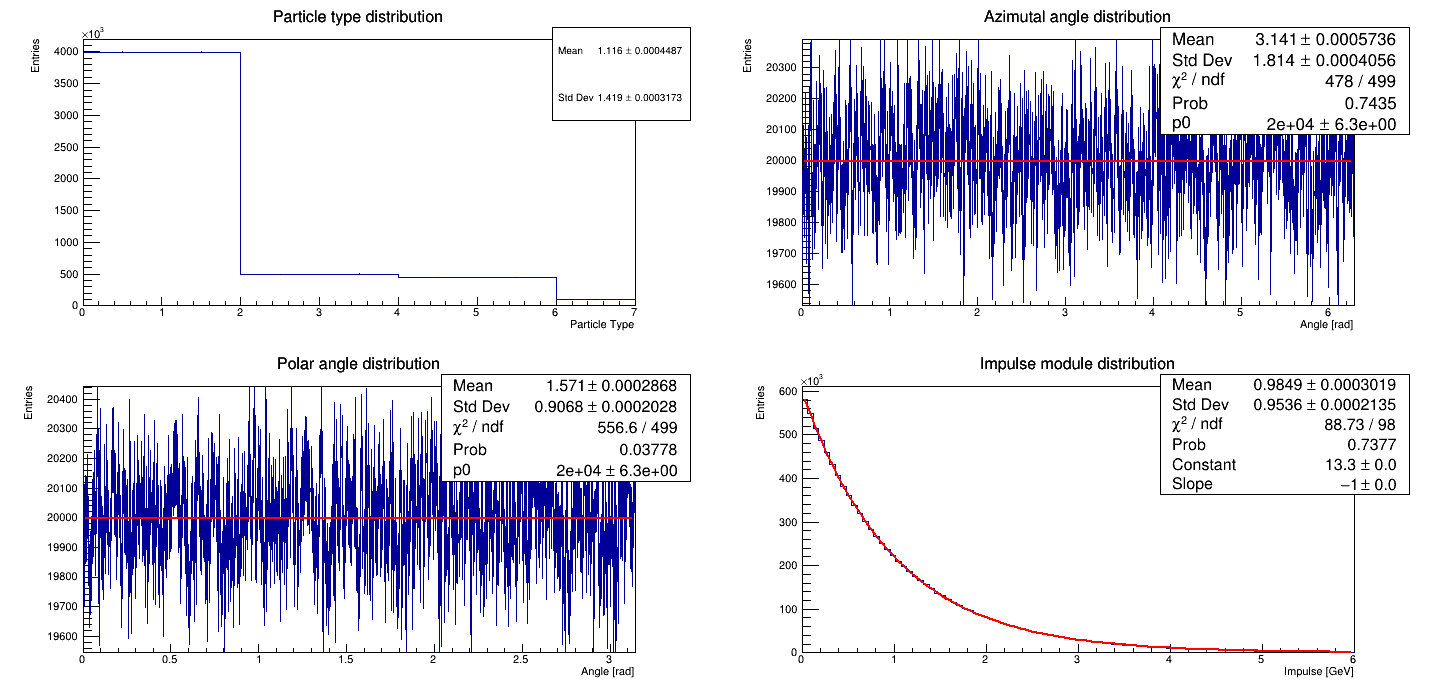
\includegraphics[width=\textwidth]{image/canvas1.png}
    \caption{\small Le distribuzioni rispettivamente (da sinistra a destra, da sopra a sotto) del numero di particelle per tipo, dell'angolo azimutale $\phi$, dell'angolo polare $\theta$ e dell'impulso. Se presenti, le curve rosse rappresentano il fit della funzione.}
    \label{fig:canvas1}
\end{figure}

In seguito nella tabella \ref{tab:ang_imp} si riportano i risultati relativi alla distribuzione dei fit degli angoli polari e azimutali e del modulo dell'impulso. In figura \ref{fig:canvas1} si osserva che le distribuzioni degli angoli sono uniformi, mentre la distribuzione dell'impulso è di decadimento esponenziale, come previsto nella sezione precedente.

\begin{table}[htp]
    \centering
    \begin{tabular}{||c|c|c|c|c||}
        \hline \hline
        \multicolumn{5}{||c||}{\textsc{analisi dei fit degli angoli $\phi$, $\theta$ e dell'impulso}} \\
        \hline \hline
        distribuzione & parametri & $\chi^2$ & DoF & $\chi^2/$DoF \\
        \hline
        angolo azimutale $\phi$ (unif.) & 19999.0 ± 6.3 & 477.97 & 499 & 0.957856\\
        angolo polare $\theta$ (unif.) & 19998.9 ± 6.3 & 556.553 & 499 & 1.11534\\
        modulo impulso (exp.) & 1.00019 ± 0.00033 & 88.7283 & 98 & 0.905391\\
        \hline \hline 
    \end{tabular}
    \caption[\small Distribuzione angoli e impulso]{\small Valori estratti dal fit delle distribuzioni dell'angolo azimutale $\phi$, dell'angolo polare $\theta$ e del modulo dell'impulso delle particelle generate.}
    \label{tab:ang_imp}
\end{table}

Nel prossimo passaggio il programma cerca di rilevare il segnale generato da K$^*$ dalle distribuzioni della massa invariante.\\
Per far ciò, vogliamo estrarre solo la massa invariante tra particelle generate da K$^*$ che sappiamo essere una coppia di K e $\pi$ di carica opposta. È possibile rilevare ciò facendo una differenza della distribuzione della massa invariante fra cariche discordi da quelle concordi, eliminando così il rumore generato tra combinazioni accidentali. Per aumentare l'efficienza della rilevazione basta sottrarre la distribuzione di masse invarianti di K e $\pi$ concordi da quelli discordi.\\
In tabella \ref{tab:massinv} si trovano i risultati dei fit di queste differenze, messa in confronto con la distribuzione di massa invariante facente da benchmark, che rappresenta la distribuzione migliore del segnale di K$^*$. Si nota come i valori della media e del sigma si avvicinano rispettivamente ai valori della massa e della larghezza di risonanza di K$^*$. Si possono inoltre visualizzare queste distribuzioni in figura \ref{fig:canvas2}.

\begin{table}[htp]
    \centering
    \begin{tabular}{||c|c|c|c|c||}
        \hline \hline
        \multicolumn{5}{||c||}{\textsc{analisi del fit di K$^*$}} \\
        \hline \hline
        distribuzione & media & sigma & ampiezza & $\chi^2/$DoF \\
        \hline
        massa inv. best & 0.89155 ± 0.00016 & 0.05084 ± 0.00012 & 23363 ± 91 & 1.47239\\
        massa inv. totale & 0.887 ± 0.011 & 0.0349 ± 0.0098 & (10.1 ± 2.4) $\cdot 10^3$ & 0.859503\\
        massa inv. K e $\pi$ & 0.8778 ± 0.0080 & 0.0443 ± 0.0070 & (7.4 ± 1.1) $\cdot 10^3$ & 0.827187\\
        \hline \hline 
    \end{tabular}
    \caption[\small Distribuzioni massa invariante]{\small Valori estratti dal fit delle distribuzioni della massa invariante migliore (“best"), della differenza tra cariche discordi e quelli concordi (“totale") e della differenza tra K e $\pi$ di carica discorde e concorde (“K e $\pi$").}
    \label{tab:massinv}
\end{table}

\begin{figure}[htbp]
    \centering
    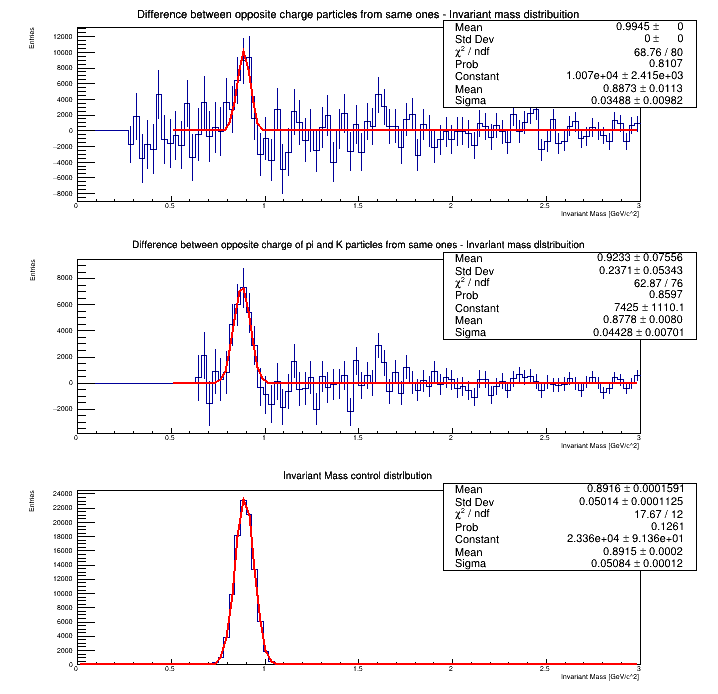
\includegraphics[width=.8\textwidth]{image/canvas2.png}
    \caption{\small Le distribuzioni rispettivamente della differenza della massa invariante tra particelle di carica opposta e concorde, tra K e $\pi$ di carica opposta e concorde e infine della differenza di massa invariante migliore.}
    \label{fig:canvas2}
\end{figure}

\newpage
\section*{Appendice}
\appendix

\section{\texttt{ParticleType.hpp}}
\input{code/ParticleType.hpp}   

\section{\texttt{ParticleType.cpp}}
\input{code/ParticleType.cpp}

\section{\texttt{ResonanceType.hpp}}
\input{code/ResonanceType.hpp}

\section{\texttt{ResonanceType.cpp}}
\input{code/ResonanceType.cpp}

\section{\texttt{Particle.hpp}}
\input{code/Particle.hpp}

\section{\texttt{Particle.cpp}}
\input{code/Particle.cpp}

\section{\texttt{main.cpp}}
\documentclass{article}

% pacchetti
\usepackage[utf8]{inputenc} 
\usepackage[italian]{babel}
\usepackage{url}
\usepackage{hyperref}
\usepackage{xcolor}
\usepackage{graphicx} % per le immagini
\usepackage{amsthm}
\usepackage{amsmath}
\usepackage{amssymb}
\usepackage{wrapfig} % per le immagini incorniciate con il testo
\usepackage{fancyhdr} % per i headings e footers
\usepackage{eurosym} % per il simbolo dell'euro "€" più carino
\usepackage{appendix}
\usepackage{geometry}
\usepackage{extpfeil}
\usepackage{tikz}
%\usetikzlibrary{patterns,plotmarks} %per usare root con tikz
\usepackage{multirow}
\usepackage{multicol} % per avere elenchi a più colonne
\usepackage{enumitem}
\usepackage{soul} % per highlight migliore

\usepackage{minted}
\definecolor{bg}{rgb}{0.95,0.95,0.95}
\definecolor{green}{rgb}{0,.66,0}
\definecolor{white}{rgb}{1, 1, 1}


% impostazioni del pacchetto fancyhdr
\pagestyle{fancy}
\fancyhf{}
\rhead{\sc ye leandro}
\lhead{Relazione \texttt{ROOT\textunderscore project}}
\fancyfoot[c]{\thepage}

\begin{document}


%\thispagestyle{plain} % per ignorare per questa pagina le impostazioni fancy
\thispagestyle{empty} % per disattivare per questa pagina le impostazioni fancy e anche il numero della pagina

\begin{figure}[h]
    \centering
    \includegraphics[width=0.5\textwidth]{image/logo.png}
    \label{Logo}
\end{figure}

\vspace{2cm}

\section*{\centering \Huge \bf Relazione \texttt{ROOT\textunderscore project}}

\vspace{3cm}

\begin{center}
{\large Realizzato da} \\
\vspace{2cm}
{\Large \textsc{Leandro Ye}}    
\end{center}

\vspace{3cm}

\begin{center}
    {\large 8 aprile 2023}
\end{center}

\newpage

\section{Introduzione}

Nella seguente relazione si intende simulare eventi di collisioni tra vari tipi di particelle e fare analisi di dati a riguardo. Per la realizzazione del programma si è utilizzato il linguaggio C++ con la libreria ROOT, con particolare enfasi sulla programmazione ad oggetti, sulla simulazione di eventi fisici tramite generazione Monte Carlo e infine sull'analisi con ROOT.\\

I tipi di particelle coinvolte posso essere raggruppati in due categorie: quelli stabili e quelli molto instabili, ossia risonanze. Per lo scopo di questo progetto, di queste particelle andiamo a considerare solo queste caratteristiche: massa, carica, quantità di moto. Solo alle risonanze però si associa un'altra caratteristica, la larghezza di risonanza. Inoltre le particelle considerate sono: pioni ($\pi^\pm$), kaoni (K$^\pm$), protoni (p$^\pm$) e infine K$^*$, con K$^*$ la particella di risonanza. \\

Nel corso delle interazioni tra queste particelle, emergeranno i parametri di K$^*$, e lo scopo di questo progetto è riuscire a determinare questi parametri.\\

\section{Struttura del codice} 

In questo progetto si è andati ad utilizzare la programmazione ad oggetti, e più in particolare l'\textbf{ereditarietà virtuale} e l'\textbf{aggregazione}.

\subsection*{Le classi \texttt{ParticleType} e \texttt{ResonanceType}}
Nella simulazione si hanno due categorie di particelle: quelli ordinari e le risonanze. Avendo queste ultime una caratteristica aggiuntiva rispetto a quelle ordinarie (cioè la larghezza di risonanza), allora si è pensato di creare una classe \verb|ParticleType| associato ai tipi particelle ordinarie e da questa si è andati a ereditare la classe \verb|ResonanceType|, associata alla tipologia di risonanza. \verb|ParticleType| possiede \textbf{tre attributi privati}:
\begin{itemize}
    \item \verb|std::string fName|: indica il \textbf{nome} del tipo di particella;
    \item \verb|double fMass|: indica il valore di \textbf{massa} (in GeV/c$^2$);
    \item \verb|int fCharge|: indica il valore di \textbf{carica} ($\pm$\textit{e}).
\end{itemize}
\verb|ResonanceType| include anche l'attributo privato \verb|double fWidth| che indica la \textbf{larghezza}.\\
Per ognuno di questi parametri c'è un metodo che ritorna il valore se richiesto (\verb|GetName()|, \verb|GetMass()|, \verb|GetCharge()|, \verb|GetWidth()|).

\subsection*{La classe \texttt{Particle}}

Alla generazione di una particella dobbiamo specificare le sue caratteristiche di base e le proprietà cinematiche (quantità di moto e direzione). Per far ciò si potrebbero attribuire le singole caratteristiche associato al tipo di particella, ma ciò è dispendioso per la memoria ed è meglio attribuire semplicemente il tipo di particella.\\

Utilizzando l'aggregazione del codice si è creato una classe \verb|Particle| che descrive queste caratteristiche, contenendo in privato:
\begin{itemize}
    \item \verb|static std::vector<ParticleType> fParticleType|: una \textbf{lista} (contenitore) di tutti i tipi di particelle creati;
    \item \verb|int fIndex|: un \textbf{numero} che identifica la tipologia di particella in base alla sua posizione in \verb|fParticleType|;
    \item \verb|Vector3d fImpulse|: un \textbf{vettore 3-dim} che racchiude i tre componenti dell'impulso.
\end{itemize}
Inoltre in questa classe troviamo diversi metodi, sia privati che pubblici:
\begin{itemize}
    \item metodi che ritornano i parametri singoli della particella corrente (indice del tipo di particella, vettore dell'impulso, massa, carica);
    \item metodi che impostano i parametri alla particella corrente (tipo di particella, impulso);
    \item \verb|int FindParticle(...)|: ritorna l'indice del tipo della particella in base al nome dato in input;
    \item \verb|void AddParticleType(...)|: aggiunge un tipo di particella in \verb|fParticleType|;
    \item \verb|double GetEnergy()|: ritorna il valore dell'energia della particella corrente, secondo l'equazione
    
    $$ E = \sqrt{m^2 + |\Vec{p}|^2} $$
    
    con $E$ l'energia, $m$ la massa, $|\Vec{p}|$ il modulo dell'impulso;
    \item \verb|double InvMass(...)|: ritorna il valore della massa invariante tra quella corrente e un'altra particella, secondo
    
    $$ M_{inv} = \sqrt{(E_1 + E_2)^2 - (\vec{p_1} + \vec{p_2})^2} $$
    
    con $M_{inv}$ la massa invariante, $E_i$ e $\Vec{p_i}$ rispettivamente l'energia e vettore dell'impulso della particella $i$;
    \item \verb|double Decay2Body(...)|: simula il decadimento della particella corrente in altre due; 
\end{itemize}

Un altro punto fondamentale di questo progetto è la \textbf{modularità} del codice: per ogni classe sono stati definiti un file di intestazione e uno d'implementazione (quindi 6 file complessivamente), che, una volta compilati, sono stati resi come librerie dinamiche per un maggior efficacia nel fase del linking.\\

\subsection*{Il file \texttt{main.cpp}}

Le librerie create sono stati utilizzati nel file \verb|main.cpp|, in cui si esegue la parte di simulazione del programma.\\
Ciò consiste in simulazione di eventi di collisione in cui vengono generati un numero fisso di particelle (\verb|Particle|) per evento. Per ogni generazione di  particella le vengono attribuite casualmente un impulso con direzione e verso (\verb|fImpulse|), le viene assegnato la tipologia di particella (\verb|fIndex|) secondo una distribuzione definita dall'utente e infine, se viene generato una risonanza, questa viene fatto decadere in altre due.\\
Durante le generazioni in un evento vengono raccolti dati in istogrammi che poi andranno ad essere analizzati successivamente. I dati che vengono raccolti di una particella generata sono il tipo di particella, la distribuzione degli angoli dell'impulso (azimutale e polare), il modulo dell'impulso totale e trasversa e l'energia. Alla fine di un evento vengono valutati anche le masse invarianti tra le particelle, in particolare quelle derivanti tra tutte le particelle, tra tutte le particelle di segno concorde e di segno opposto, tra particelle K e $\pi$ di segno concorde  e di segno opposto e infine tra particelle entrambi generate da uno stesso decadimento di un K$^*$. 
Alla fine dell'esecuzione del programma vengono mostrati e salvati i dati della simulazione effettuata.\\

\subsection*{Il file \texttt{analytics.cpp}}
Infine, una volta salvati i dati della simulazione, questi vengono analizzati e fittati.
In particolare vengono analizzati e valutati il numero di particelle generati per tipo, i parametri della particella (angoli e modulo dell'impulso) e le masse invarianti. Da queste analisi si cerca di rilevare il segnale di K$^*$ che verrà generato con frequenza molto minore rispetto ad altre particelle.\\

\section{Generazione}

Nel programma vengono generati 10 000 eventi, in ognuno dei quali vengono generati 100 particelle.\\
Le particelle in totale sono 7, con i tipi, le caratteristiche e la distribuzione delle particelle generate raccolte nella tabella \ref{tab:particles}.

\begin{table}[htp]
    \centering
    \begin{tabular}{||c|c|c|c|c||}
        \hline \hline
        \multicolumn{5}{||c||}{\textsc{tipo, caratteristiche e distribuzione delle particelle}} \\
        \hline \hline
        tipo & presenza & massa [GeV/c$^2$] & carica [$e$] & larghezza [GeV/c$^2$]\\
        \hline
        $\pi^\pm$ & 40\% & 0.13957 & $\pm1$ & $-$\\
        K$^\pm$ & 5\% & 0.49367 & $\pm1$ & $-$\\
        p$^\pm$ & 4.5\% & 0.93827 & $\pm1$ & $-$\\
        K$^*$ & 1\% & 0.89166 & 0 & 0.050\\
        \hline \hline 
    \end{tabular}
    \caption[\small Tipo, caratteristiche e distribuzione delle particelle]{\small Il tipo, le caratteristiche e la loro distribuzione nelle simulazioni, con $\pi^\pm$ pioni, K$^\pm$ kaoni, p$^\pm$ protoni e  K$^*$ la particella di risonanza. La sezione "presenza" indica la distribuzione nella simulazione per evento.}
    \label{tab:particles}
\end{table}
Per quanto riguarda invece l'impulso $\Vec{p}$ delle particelle il suo modulo segue una distribuzione esponenziale decrescente con media $<|\Vec{p}|>$ = 1 GeV, mentre la distribuzione degli angoli (in coordinate sferiche) seguono secondo lo schema:
\begin{itemize}
    \item angolo azimutale $\phi$ con distribuzione uniforme tra [0, $2\pi$];
    \item angolo polare $\theta$ con distribuzione uniforme tra [0, $\pi$];
\end{itemize}
Nel caso in cui la particella generata sia un K$^*$, questa, prima della raccolta dati, decade subito in altre due particelle che possono essere o un $\pi^+$ e un K$^-$, oppure un $\pi^-$ e un K$^+$, con probabilità 50\% in entrambi i casi. Queste due particelle inoltre, attraverso la funzione \verb|Decay2Body(...)|, assumono un impulso casuale ciascuno ma tale che siano rispettate le leggi della fisica. Inoltre ciò vuol dire che al termine di un evento si possono aver più di 100 particelle. 

\section{Analisi}

Dopo l'esecuzione del programma di \verb|analytics.cpp|
ci vengono forniti i risultati dei dati.
Nella tabella \ref{tab:types} vengono forniti il numero di particelle generate per tipo. Si noti che non sono state contate le particelle generate da K$^*$.\\ Nell'istogramma in alto a sinistra della figura \ref{fig:canvas1} è possibile visualizzare tale distribuzione.

\begin{table}[htp]
    \centering
    \begin{tabular}{||c|c|c||}
        \hline \hline
        \multicolumn{3}{||c||}{\textsc{occorrenze}} \\
        \hline \hline
        tipo & osservate & attese \\
        \hline
        $\pi^+$ & $ (3998.0 \pm 2.0) \cdot 10^3$ & $4000 \cdot 10^3$\\
        $\pi^-$ & $ (3999.0 \pm 2.0) \cdot 10^3$ & $4000 \cdot 10^3$\\
        K$^+$ & $ (5002.5 \pm 7.1) \cdot 10^2$ & $5000 \cdot 10^2$\\
        K$^-$ & $ (5009.3 \pm 7.1) \cdot 10^2$ & $5000 \cdot 10^2$\\
        p$^+$ & $ (4509.9 \pm 6.7) \cdot 10^2$ & $4500 \cdot 10^2$\\
        p$^-$ & $ (4515.5 \pm 6.7) \cdot 10^2$ & $4500 \cdot 10^2$\\
        K$^*$ & $ (992.6 \pm 3.2) \cdot 10^2$ & $1000 \cdot 10^2$\\
        \textsc{tot} & $ (10000 \pm 3.2) \cdot 10^3$ & $10000 \cdot 10^3$\\
        \hline \hline 
    \end{tabular}
    \caption[\small Occorrenze delle particelle]{\small Numero di particelle osservate e attese per tipo di particella e quella totale (“\textsc{tot}"). NOTA: L'incertezza di \textsc{tot} è ottenuto per conteggio diretto del programma, non per propagazione degli errori.}
    \label{tab:types}
\end{table}

\begin{figure}[htbp]
    \centering
    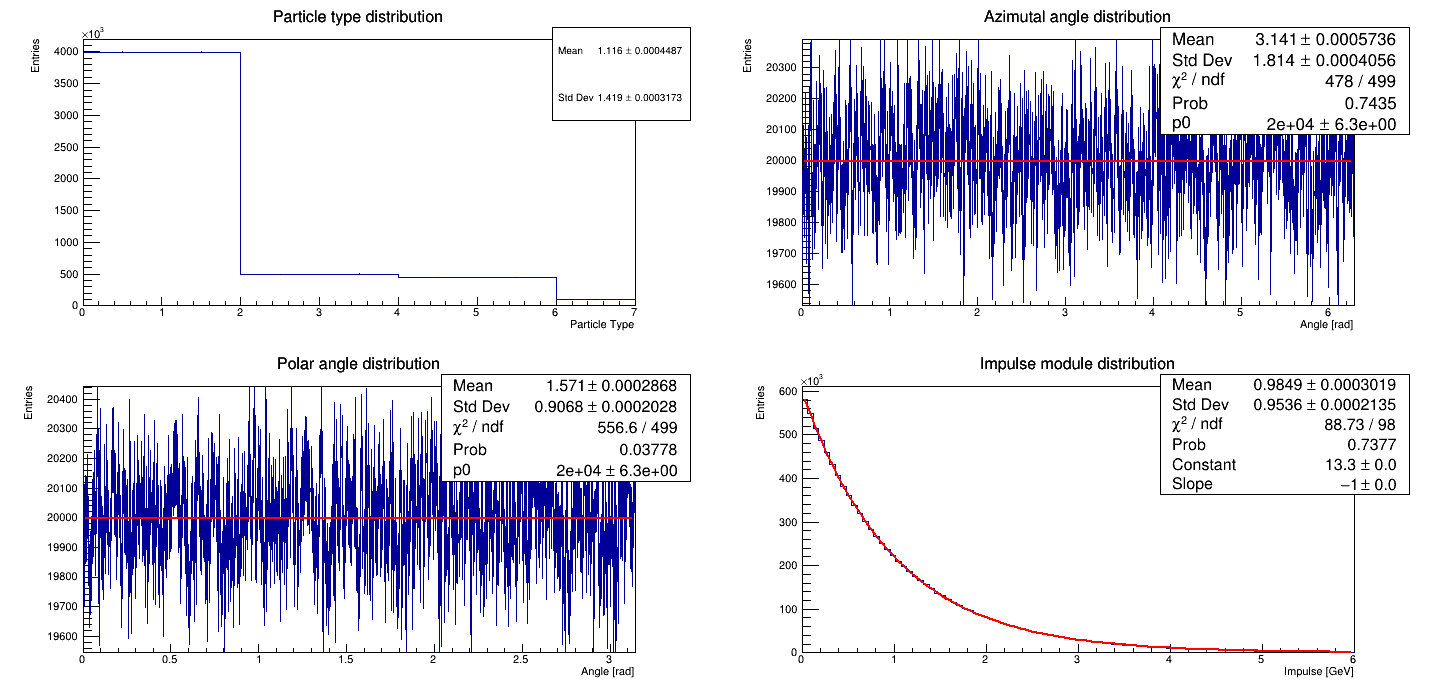
\includegraphics[width=\textwidth]{image/canvas1.png}
    \caption{\small Le distribuzioni rispettivamente (da sinistra a destra, da sopra a sotto) del numero di particelle per tipo, dell'angolo azimutale $\phi$, dell'angolo polare $\theta$ e dell'impulso. Se presenti, le curve rosse rappresentano il fit della funzione.}
    \label{fig:canvas1}
\end{figure}

In seguito nella tabella \ref{tab:ang_imp} si riportano i risultati relativi alla distribuzione dei fit degli angoli polari e azimutali e del modulo dell'impulso. In figura \ref{fig:canvas1} si osserva che le distribuzioni degli angoli sono uniformi, mentre la distribuzione dell'impulso è di decadimento esponenziale, come previsto nella sezione precedente.

\begin{table}[htp]
    \centering
    \begin{tabular}{||c|c|c|c|c||}
        \hline \hline
        \multicolumn{5}{||c||}{\textsc{analisi dei fit degli angoli $\phi$, $\theta$ e dell'impulso}} \\
        \hline \hline
        distribuzione & parametri & $\chi^2$ & DoF & $\chi^2/$DoF \\
        \hline
        angolo azimutale $\phi$ (unif.) & 19999.0 ± 6.3 & 477.97 & 499 & 0.957856\\
        angolo polare $\theta$ (unif.) & 19998.9 ± 6.3 & 556.553 & 499 & 1.11534\\
        modulo impulso (exp.) & 1.00019 ± 0.00033 & 88.7283 & 98 & 0.905391\\
        \hline \hline 
    \end{tabular}
    \caption[\small Distribuzione angoli e impulso]{\small Valori estratti dal fit delle distribuzioni dell'angolo azimutale $\phi$, dell'angolo polare $\theta$ e del modulo dell'impulso delle particelle generate.}
    \label{tab:ang_imp}
\end{table}

Nel prossimo passaggio il programma cerca di rilevare il segnale generato da K$^*$ dalle distribuzioni della massa invariante.\\
Per far ciò, vogliamo estrarre solo la massa invariante tra particelle generate da K$^*$ che sappiamo essere una coppia di K e $\pi$ di carica opposta. È possibile rilevare ciò facendo una differenza della distribuzione della massa invariante fra cariche discordi da quelle concordi, eliminando così il rumore generato tra combinazioni accidentali. Per aumentare l'efficienza della rilevazione basta sottrarre la distribuzione di masse invarianti di K e $\pi$ concordi da quelli discordi.\\
In tabella \ref{tab:massinv} si trovano i risultati dei fit di queste differenze, messa in confronto con la distribuzione di massa invariante facente da benchmark, che rappresenta la distribuzione migliore del segnale di K$^*$. Si nota come i valori della media e del sigma si avvicinano rispettivamente ai valori della massa e della larghezza di risonanza di K$^*$. Si possono inoltre visualizzare queste distribuzioni in figura \ref{fig:canvas2}.

\begin{table}[htp]
    \centering
    \begin{tabular}{||c|c|c|c|c||}
        \hline \hline
        \multicolumn{5}{||c||}{\textsc{analisi del fit di K$^*$}} \\
        \hline \hline
        distribuzione & media & sigma & ampiezza & $\chi^2/$DoF \\
        \hline
        massa inv. best & 0.89155 ± 0.00016 & 0.05084 ± 0.00012 & 23363 ± 91 & 1.47239\\
        massa inv. totale & 0.887 ± 0.011 & 0.0349 ± 0.0098 & (10.1 ± 2.4) $\cdot 10^3$ & 0.859503\\
        massa inv. K e $\pi$ & 0.8778 ± 0.0080 & 0.0443 ± 0.0070 & (7.4 ± 1.1) $\cdot 10^3$ & 0.827187\\
        \hline \hline 
    \end{tabular}
    \caption[\small Distribuzioni massa invariante]{\small Valori estratti dal fit delle distribuzioni della massa invariante migliore (“best"), della differenza tra cariche discordi e quelli concordi (“totale") e della differenza tra K e $\pi$ di carica discorde e concorde (“K e $\pi$").}
    \label{tab:massinv}
\end{table}

\begin{figure}[htbp]
    \centering
    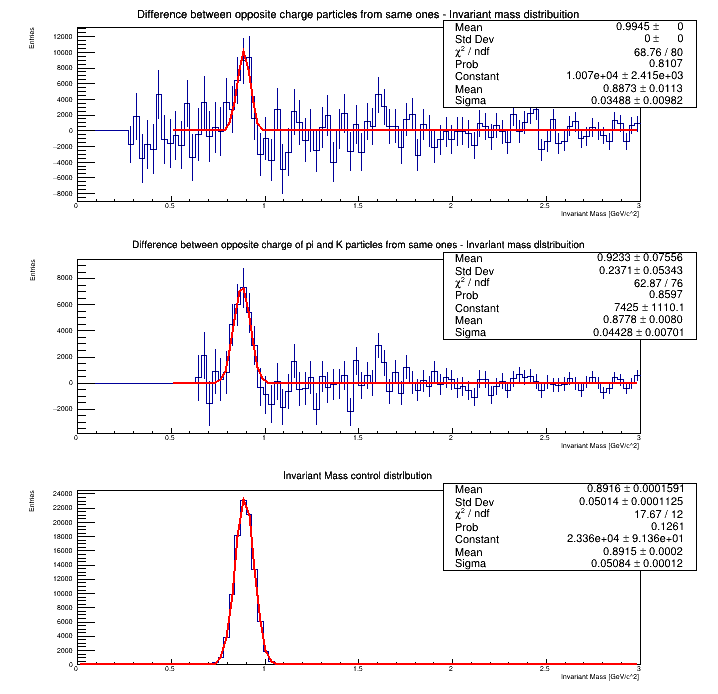
\includegraphics[width=.8\textwidth]{image/canvas2.png}
    \caption{\small Le distribuzioni rispettivamente della differenza della massa invariante tra particelle di carica opposta e concorde, tra K e $\pi$ di carica opposta e concorde e infine della differenza di massa invariante migliore.}
    \label{fig:canvas2}
\end{figure}

\newpage
\section*{Appendice}
\appendix

\section{\texttt{ParticleType.hpp}}
\input{code/ParticleType.hpp}   

\section{\texttt{ParticleType.cpp}}
\input{code/ParticleType.cpp}

\section{\texttt{ResonanceType.hpp}}
\input{code/ResonanceType.hpp}

\section{\texttt{ResonanceType.cpp}}
\input{code/ResonanceType.cpp}

\section{\texttt{Particle.hpp}}
\input{code/Particle.hpp}

\section{\texttt{Particle.cpp}}
\input{code/Particle.cpp}

\section{\texttt{main.cpp}}
\input{code/main.cpp}

\section{\texttt{analytics.cpp}}
\input{code/analytics.cpp}

\end{document}

\section{\texttt{analytics.cpp}}
\input{code/analytics.cpp}

\end{document}